% !TEX encoding = UTF-8
% !TEX TS-program = pdflatex
% !TEX root = ../tesi.tex

%**************************************************************
\chapter{Architettura per computazione parallela}
\label{cap:architettura-computazione-parallela}
%**************************************************************

La precedente architettura risponde all'esigenza di stabilire una comunicazione cross-page, ma lascia irrisolti diversi obiettivi del progetto. In questo capitolo viene invece presentata un'evoluzione di tale architettura, al fine di poter migliorare le performance di \textit{Stargate} ed offrire un sistema di gestione dei widget più indipendente.
Dal punto di vista delle performance, non è difatti sufficiente eseguire le nuove finestre in un processo separato. Sarebbe infatti più ottimale che il calcolo dello \textbf{stato derivato} venga effettuato una volta sola per tutti i widget della stessa tipologia.

\section{Stato derivato}

Per \textit{stato derivato} si intende l'insieme dei dati, calcolati a partire dallo stato applicativo dell'applicazione, necessari al widget per la corretta esecuzione di tutte le sue funzionalità. La funzione che calcola tali dati, avente per input lo stato applicativo e per output lo stato derivato, viene convenzionalmente denominata \textbf{selector} ed ha una firma di tipo \texttt{State => DerivedState}.

Tutte le funzioni \textit{selectors} devono inoltre essere pure \footnote{\url{https://en.wikipedia.org/wiki/Pure_function}}, ovvero ritornare lo stesso risultato a parità di input e non avere effetti collaterali (\textit{side-effects}), quali accesso/modifica a variabili non locali alla funzione, modifiche per riferimenti, accesso a I/O etc. \\

Nel seguente esempio lo stato applicativo rappresenta un'applicazione che gestisce una lista di acquisti. Si immagini quindi di avere un widget UI per mostrare il totale delle spese e che quindi necessiti di tale stato derivato.

\begin{lstlisting}[language={[Sharp]C},basicstyle=\footnotesize]
interface Purchase {
    name: number
    price: number
}

interface State {
    purchases: Array<Purchase>
}

type DerivedState = number

function sumSelector(state: State): DerivedState {
    let sum: number = 0;

    for (let i = 0; i < state.purchases.length; i++) {
        sum += state.purchases[i].price;
    }

    return sum
}
\end{lstlisting}

Essendo funzioni pure, è possibile comporre \textit{selectors} nella stessa maniera in cui si compongono funzioni matematiche \texttt{f ° g}, ottenendo \textit{selectors} più complessi ma comunque modulari. Il \textit{selector} finale di un componente UI può essere il risultato di decine di sotto-\textit{selectors}, a loro volte composti da altri \textit{selectors}.

\begin{figure}[H] 
  \centering 
  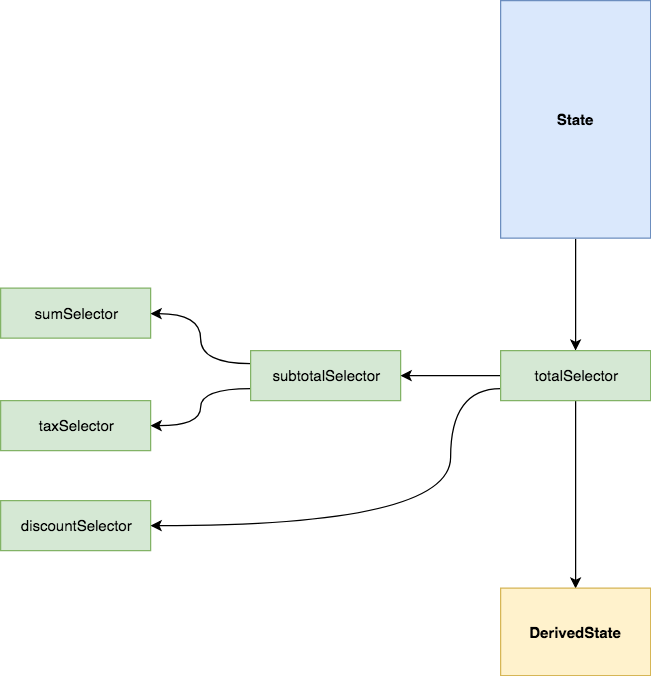
\includegraphics[width=1\columnwidth]{selectors} 
  \caption{Esempio di composizione di selectors}
\end{figure}

È facile quindi immaginare che in un componente UI complesso quale una mappa dei veicoli e rotte, tali \textit{selectors} siano molto complessi e richiedano un tempo di computazione non indifferente. \\

In particolare il codice JavaScript dell'applicazione principale è eseguito in un unico thread, per cui calcolare nell'applicazione padre lo stato derivato di diverse finestre con mappe potrebbe bloccare l'applicazione e renderla incapace di rispondere alle interazioni utenti fino al termine dei calcoli nei \textit{selectors}. \\

Una possibile soluzione potrebbe essere delegare tale calcolo nelle finestre figlie, poiché vivono su processi dedicati. Sebbene sia accettabile, non è ottimale in quanto il calcolo dei \textit{selectors} sarebbe ripetuto pur essendo identico per due finestre aventi entrambe la stessa tipologia di widget, per cui esiste un'alternativa migliore. \\

L'ideale è difatti calcolare lo stato derivato per ciascun tipo di widget una sola volta ad ogni modifica dello stato applicativo e propagare il risultato del calcolo ai widget, ad esempio a tutte le finestre contenenti la mappa. In tal modo l'onere computazionale è linearmente dipendente dal numero di \textbf{tipi di widget} attivi invece che dal numero totale di finestre. Tuttavia tale calcolo allo stesso tempo non può avvenire nella finestra padre per le stesse ragioni descritte sopra riguardo al eseguirlo in quelle figlie.

\section{Web Worker}\label{webworker}

\begin{figure}[H] 
  \centering 
  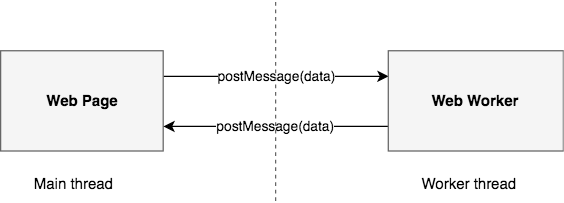
\includegraphics[width=1\columnwidth]{worker} 
  \caption{Comunicazione tra la pagine web ed il Web Worker}
\end{figure}

Un \textit{Web Worker} è un modo per una pagina web di eseguire del codice in un thread background, in grado di eseguire attività senza interferire con l'interfaccia utente. Nello specifico è un oggetto della classe \texttt{Worker}, creato passando come parametro il file che contiene il codice da eseguire nel thread separato. Tale thread non avrà alcun riferimento di memoria in comune con il main thread della pagina e viene considerato come un contesto di esecuzione separato. \\

È possibile eseguire qualsiasi tipo di codice all'interno del thread worker, con alcune eccezioni tuttavia. Ad esempio non è possibile manipolare direttamente i nodi HTML della pagina web o accedere ad API CSS/HTML. In generale un \textit{Web Worker} è da considerare un thread di calcolo computazione e non di manipolazione della pagina. \\

Un aspetto positivo è invece il sistema di comunicazione tra il worker e il thread principale dell'applicazione web, in quanto avviene anch'esso via \textit{postMessage} come se fosse tra finestre. Infine i \textit{Web Workers} possono attivare nuovi workers per delegare ulteriormente del lavoro in nuovi threads. \\

È quindi chiaro che un \textit{Web Worker} è il candidato ideale in \textit{Stargate} per l'esecuzioni dei \textit{selectors}. Nello specifico si desidera calcolare in un thread apposito lo stato derivato per ciascuna tipologia di widget, salvarla in cache ed inviarla a tutti i widget attivi di tale tipologia. Salvando in cache, è possibile renderizzare istantaneamente un widget alla sua apertura in quanto lo stato derivato necessario è stato già calcolato precedentemente.

Inoltre, poiché i calcoli avvengono in un thread di background, non vi sono impatti negativi nelle performance sia dell'applicazione principale che delle finestre widget. \\

Purtroppo l'utilizzo del \textit{Web Worker} genera un nuovo problema: le nuove finestre devono essere aperte comunque dalla pagina principale in quanto le relative API non sono disponibili nel Worker, ma non è quindi possibile per questi ottenerne i riferimenti per poter usare \texttt{widgetWindow.postMessage(derivedState)}. 

\section{BroadcastChannel}

Un \textit{BroadcastChannel} è un canale di comunicazione broadcast tra diversi "contesti" del browser (ad esempio finestre, tabs o workers) provenienti dallo stesso sito. È difatti disponibile anche da parte dei \textit{Web Workers}. \\

Creando un \textit{BroadcastChannel}, il quale rimane in ascolto del sottostante canale di comunicazione, si è in grado di inviare messaggi attraverso di esso usando \texttt{channel.postMessage(data)}, dunque usando il riferimento all'istanza di \textit{BroadcastChannel} invece che della finestra. Allo stesso tempo è possibile rimanere in ascolto di tutti i messaggi inviati attraverso il canale ed ogni messaggio è inviato a tutti coloro in ascolto, ovvero in broadcast. \\

È possibile quindi comunicare tra le parti senza riferimenti reciproci. Ogni parte dell'architettura è in grado di sottoscriversi al canale \textit{BroadcastChannel} ed avere una comunicazione bi-direzionale (\textit{full-duplex}) verso tutte le altre.

\begin{figure}[H] 
  \centering 
  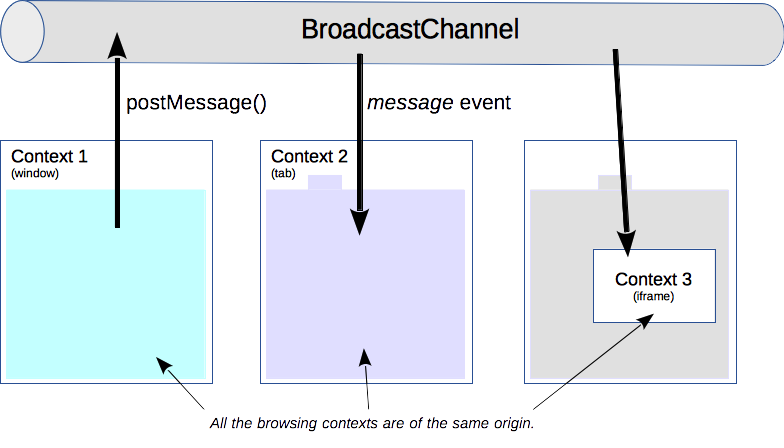
\includegraphics[width=1\columnwidth]{BroadcastChannel} 
  \caption{Esempio di funzionamento del BroadcastChannel}
\end{figure}

\section{Evoluzione architettura Stargate}

Alla luce degli aggiornamenti sui \textit{Web Workers} e sul \textit{BroadcastChannel}, si presenta la nuova architettura del progetto \textit{Stargate}.

\begin{figure}[H] 
  \centering 
  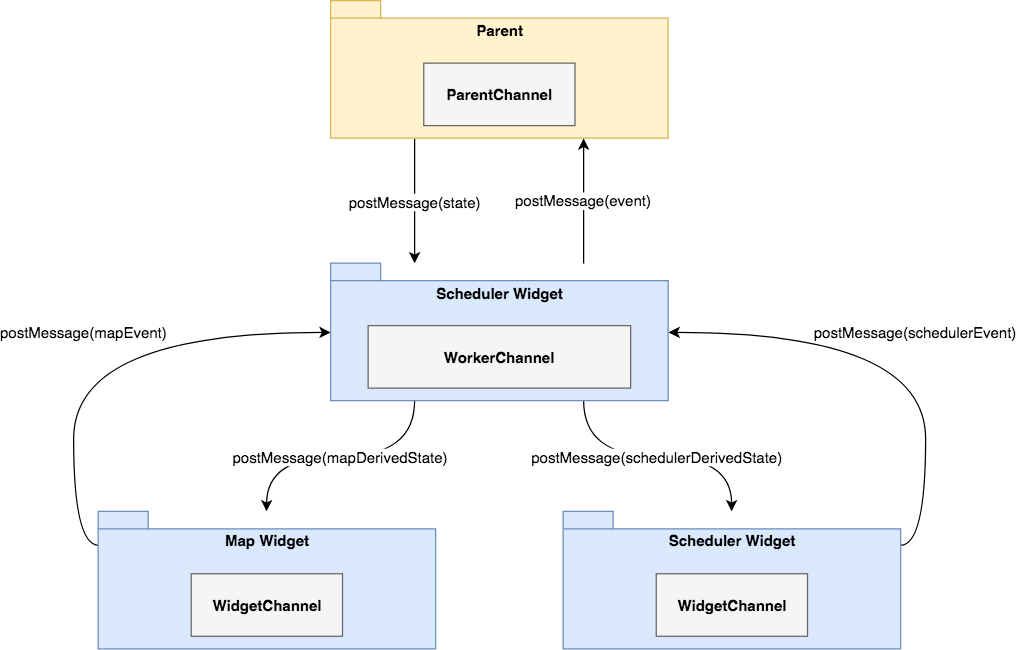
\includegraphics[width=1\columnwidth]{architettura2} 
  \caption{Architettura Stargate evoluta con Web Worker e BroadcastChannel}
\end{figure}

Le classi \textit{Parent} e \textit{Widget} sono divenute ora packages, in quanto contengono altre classi sottostanti tra cui quelle che gestiscono la comunicazione tramite \textit{BroadcastChannel}. \\

\textbf{ParentChannel}
    \begin{itemize}
        \item vive nella finestra principale ed è unica per sessione;
        \item gestisce il canale di comunicazione \textit{BroadcastChannel} verso il \textit{Web Worker};
        \item si occupa della creazione delle finestre widget, ma manda lo stato applicativo dell'applicazione al \textit{Web Worker} e \textbf{non} conosce le esigenze dei widget, a differenza all'architettura precedente;
        \item gestisce gli eventi dei widgets che necessitano di modificare lo stato applicativo dell'applicazione.
    \end{itemize}
\textbf{WorkerChannel}
    \begin{itemize}
        \item Vive nel \textit{Web Worker}, creato dal \textit{ParentChannel};
        \item Fa da intermediario per la comunicazione tra il \textit{ParentChannel} e tutti i diversi \textit{WidgetChannel};
        \item Riceve lo stato applicativo dal \textit{ParentChannel} e fornisce gli stati derivati a ciascun widget. Lo stato derivato, ad ogni modifica dello stato applicativo, è calcolato una volta sola per ogni tipologia di widget come descritto nelle sezioni precedenti;
        \item Propaga gli eventi dai \textit{WidgetChannel} verso il \textit{ParentChannel}.
    \end{itemize}
\textbf{WidgetChannel}
    \begin{itemize}
        \item Vive in una finestra widget, creata dal \textit{Parent};
        \item Riceve lo stato applicativo dal \textit{Web Worker} ed utilizza i dati in essa per la corretta rappresentazione UI. Ogni volta che lo stato cambia, si aggiorna automaticamente anche la UI;
        \item Comunica al \textit{Web Worker} (e non direttamente al \text{Parent}) qualsiasi evento che abbia effetti sullo stato applicativo, ad esempio un'interazione utente.
    \end{itemize}
